% a=3,b=4,c=5: base AB=8; distances from O,F to x=3 are 3,2.
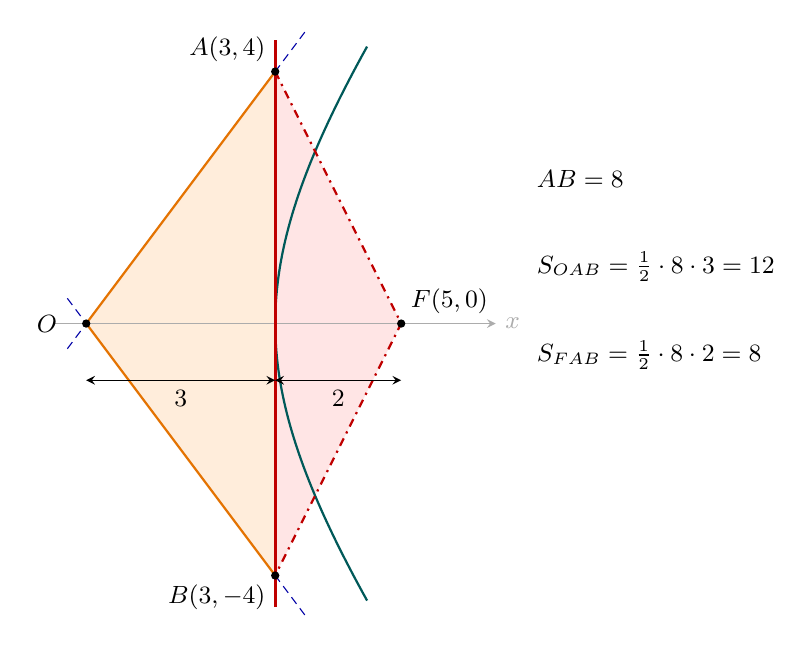
\begin{tikzpicture}[x=.8cm,y=.8cm,>=stealth,every node/.style={font=\small}]
\coordinate (O) at (0,0);\coordinate (F) at (5,0);
\coordinate (A) at (3,4);\coordinate (B) at (3,-4);
\fill[orange!14] (O)--(A)--(B)--cycle;
\fill[red!10] (F)--(A)--(B)--cycle;
\draw[gray!65,->] (-.5,0)--(6.5,0) node[right] {$x$};
\draw[blue!65!black,densely dashed] (-.3,-.4)--(3.5,4.666667);
\draw[blue!65!black,densely dashed] (-.3,.4)--(3.5,-4.666667);
\draw[teal!70!black,thick,domain=-.95:.95,samples=80,variable=\t]
 plot ({1.5*(exp(\t)+exp(-\t))},{2*(exp(\t)-exp(-\t))});
\draw[red!75!black,very thick] (3,-4.5)--(3,4.5);
\draw[orange!90!black,thick] (A)--(O)--(B);
\draw[red!75!black,thick,dash dot] (A)--(F)--(B);
\fill (O) circle(1.5pt) node[left=7pt] {$O$};
\fill (F) circle(1.5pt) node[above right] {$F(5,0)$};
\fill (A) circle(1.5pt) node[above left] {$A(3,4)$};
\fill (B) circle(1.5pt) node[below left] {$B(3,-4)$};
\draw[<->] (0,-.9)--(3,-.9) node[midway,below] {$3$};
\draw[<->] (3,-.9)--(5,-.9) node[midway,below] {$2$};
\node[anchor=west] at (7,2.3) {$AB=8$};
\node[anchor=west] at (7,.9) {$S_{OAB}=\frac12\cdot8\cdot3=12$};
\node[anchor=west] at (7,-.5) {$S_{FAB}=\frac12\cdot8\cdot2=8$};
\end{tikzpicture}
